\documentclass[conference]{IEEEtran}
\usepackage{amsmath}
\usepackage{graphicx}
\usepackage{booktabs}
\usepackage{url}

\begin{document}

\title{Beyond the Single Run: An Empirical Audit of Seed Variance, Dataset Leakage, and Statistical Power in Multi-Modality Medical Image Classification}

\author{
\IEEEauthorblockN{Aditya Ayushman Sahoo}
\IEEEauthorblockA{% Please replace with your institution/affiliation before submission.
Independent Researcher\\
Email: adityaasahoo@gmail.com}
}

\maketitle

\begin{abstract}
Reported accuracy figures for medical imaging classifiers are usually the product of one training run, one train/test split, and one evaluation metric. We treat this practice as a hypothesis rather than a given and test it against a deployed multi-modality diagnostic platform covering chest radiography, brain magnetic resonance imaging, and mammography. Repeating training across five random seeds shows that the model already in production for brain tumour classification was, by chance, the worst-performing of the five, trailing the seed mean by 2.4 accuracy points and the best seed by 3.7 points; replacing the deployed checkpoint with the better seed required no architectural change and no additional inference cost. Evaluating the same model on an independent public compilation exposes a further problem specific to reused imaging benchmarks: 63.5\% of that "independent" dataset turns out to be exact or near-duplicate copies of our own training images, discovered through byte-level and perceptual hashing rather than assumed absent. The contaminated and deduplicated evaluations score within half a point of one another, indicating the model had not memorised its training set, but the finding argues for duplicate screening as a standard step before any cross-dataset claim. A parallel experiment distils a three-model ensemble into a single deployable network and finds the student performs significantly worse than an equivalently-sized model trained directly, because the ensemble itself reaches only 87.4\% accuracy on its own training data and therefore transmits label noise rather than refined knowledge. Finally, retraining the chest radiograph classifier on the full available corpus rather than a historical subset produces a statistically significant gain in ranking ability (ROC-AUC, $p<0.0001$) that a same-sample accuracy comparison fails to detect ($p=0.449$), illustrating how metric choice alone can reverse a reported conclusion at realistic clinical sample sizes. We report all four results, including the two that returned negative outcomes, and distil them into a lightweight audit procedure that adds no new architecture and can be applied to an existing pipeline in the time it takes to rerun evaluation.
\end{abstract}

\begin{IEEEkeywords}
medical image classification, reproducibility, dataset leakage, knowledge distillation, statistical significance, deep learning evaluation
\end{IEEEkeywords}

\section{Introduction}

A deep learning classifier for a medical imaging task is typically reported with a single accuracy or area-under-curve figure, obtained from one training run evaluated on one held-out split. This convention is convenient and nearly universal, and it is also the source of several well-documented failure modes that the broader machine learning community has raised in other domains: training with different random seeds can move an architecture's ranking relative to a competing architecture \cite{picard2021}; small held-out test sets are frequently too underpowered for the metric being reported to distinguish a real effect from noise \cite{henderson2018}; and evaluation sets assembled from public repositories can silently overlap with the data a model has already seen, inflating apparent generalisation \cite{kapoor2023leakage}. In medical imaging specifically, where clinically meaningful test sets are often in the hundreds rather than the tens of thousands of images, these effects are not asymptotically negligible -- they are large enough to change which model gets deployed.

This paper is an audit rather than a new architecture. We operate a multi-modality diagnostic platform already in production, covering three independent classification tasks -- three-class chest radiograph triage, four-class brain tumour classification from magnetic resonance imaging, and binary mammography malignancy classification -- built on a shared transfer-learning recipe across four convolutional backbones. Rather than propose a new model, we subject the platform's existing evaluation practice to four specific, low-cost interventions and report exactly what each one found, including where the intervention failed to help.

The four interventions are as follows. First, every headline claim across two of the three modalities is re-evaluated across five random seeds rather than one, with means and 95\% confidence intervals reported using the same procedure throughout the paper. Second, the brain tumour classifier is evaluated zero-shot on an independent public compilation of MRI images that shares the same four-class label space -- a rare and valuable coincidence for benchmarking -- but before trusting the result, the two datasets are screened against each other with exact and perceptual image hashing, because the external compilation is documented as merging several existing sources, one of which turns out to be the very dataset used for training here. Third, a soft-voting three-model ensemble already shown to outperform any single backbone is distilled into one deployable network, testing whether an ensemble's advantage transfers to a single model at no additional inference cost, or whether distillation introduces its own failure mode when the teacher itself is imperfect. Fourth, the chest radiograph classifier -- trained historically on a five-thousand-image subset of a twenty-six-thousand-image corpus for computational reasons no longer in effect -- is retrained on the full corpus and compared against the original on the identical held-out images, using both accuracy and ROC-AUC, to see whether the two metrics agree on whether more data helped.

Two of the four interventions produced a clear improvement that has since been deployed. Two did not, and we report the negative results with the same statistical treatment as the positive ones, on the view that a negative result reached through the same rigour as a positive one is informative rather than merely disappointing. The methodological content of this paper -- how the checks were constructed, what threshold and design choices they required, and what each one cost to run -- is intended to be reusable by any team operating a similar pipeline, independent of the specific tasks or architectures involved here.

\section{Related Work}

The sensitivity of deep learning results to random seed has been documented outside medical imaging in reinforcement learning, where seed alone was shown to produce performance differences comparable to the differences between published algorithms \cite{henderson2018}, and in supervised vision tasks, where a widely cited demonstration showed that seed selection could move a model's relative ranking against a baseline it was being compared to \cite{picard2021}. Bouthillier et al. argue more broadly that variance from data splitting and seed is frequently larger than the variance the field treats as meaningful when comparing methods \cite{bouthillier2021}. Our contribution relative to this line of work is not conceptual -- the risk is known -- but empirical and specific to a clinical setting: we show a case where the seed variance was large enough that the model already serving predictions in production was outperformed by every other seed tested.

Data leakage between training and evaluation sets is an established concern in applied machine learning generally \cite{kaufman2012leakage}, and has been raised specifically for medical imaging and clinical prediction models, where Wynants et al.'s systematic review of COVID-19 prognostic models found the large majority at high risk of bias from evaluation practices including undisclosed overlap between development and validation data \cite{wynants2020}. Most treatments of this problem address leakage within a single dataset's own train/test split. The leakage we identify is a different and, we believe, under-discussed variant: two ostensibly independent public datasets, each individually documented and widely used, that overlap because one was assembled in part from the other. Kaggle-hosted compilations of pre-existing academic datasets are common in medical imaging, and our finding suggests that any claim of cross-dataset generalisation built on such a compilation should first establish, rather than assume, independence.

Knowledge distillation, introduced by Hinton et al. as a way to transfer the generalisation of a large or ensembled model into a smaller deployable one by training the student against the teacher's soft output distribution rather than hard labels alone \cite{hinton2015}, is normally reported as beneficial. We report a case in which it measurably was not, and trace the cause to a specific, checkable property of the teacher rather than treating the failure as unexplained.

Finally, our per-modality results are compared directly against published baselines evaluated on the same or closely matched datasets: a neural architecture search study on the identical brain tumour dataset used here \cite{zhang2022}, a mass-subset CBIS-DDSM mammography classifier \cite{jaamour2024}, and a chest radiograph classifier on the same RSNA pneumonia corpus \cite{valluri2023}. These comparisons are reported in Section~\ref{sec:results} alongside, not instead of, the internal audit results, since a platform's standing against the published literature and the reliability of its own internal evaluation are separate questions.

\section{Platform and Datasets}

The platform under audit serves predictions for three imaging modalities from a shared codebase. Every classifier is a convolutional backbone drawn from a common set of four architectures -- VGG16, ResNet50, DenseNet121, and EfficientNet-B0, all initialised from ImageNet weights -- fine-tuned with an identical two-phase recipe: the backbone is frozen while a newly attached classification head is trained for several epochs, after which the top fraction of the network is unfrozen and fine-tuned at a substantially lower learning rate. Early stopping, class-weighted loss, and the same preprocessing pipeline are applied uniformly across modalities, so that differences reported later in this paper reflect the data and the specific intervention under test rather than incidental differences in training procedure.

\begin{table}[t]
\centering
\caption{Dataset scale and split for each modality audited in this paper.}
\label{tab:datasets}
\begin{tabular}{lccc}
\toprule
Modality & Images & Classes & Split (train/val/test) \\
\midrule
Chest radiograph & 26{,}684 & 3 & 18{,}678 / 4{,}003 / 4{,}003 \\
Brain MRI & 3{,}264 & 4 & 2{,}284 / 490 / 490 \\
Mammography (full) & 2{,}857 & 2 & 1{,}995 / 424 / 438 \\
\bottomrule
\end{tabular}
\end{table}

The chest radiograph classifier addresses three-class triage (normal, lung opacity, and an ambiguous "no lung opacity / not normal" category) on the RSNA Pneumonia Detection Challenge corpus \cite{rsna2019}. The brain tumour classifier performs four-class discrimination (glioma, meningioma, pituitary tumour, and no tumour) on a widely used Kaggle compilation drawing in part on an earlier figshare release \cite{cheng2015}. The mammography classifier addresses binary benign/malignant discrimination on the Curated Breast Imaging Subset of the Digital Database for Screening Mammography (CBIS-DDSM) \cite{lee2017}, with a second, much older and independently sourced dataset, the Mammographic Image Analysis Society database \cite{suckling1994}, reserved for cross-dataset testing rather than training. Table~\ref{tab:datasets} summarises scale and split for the three primary training corpora; the external evaluation sets used for cross-dataset testing are introduced alongside the results that use them.

\section{Audit Methodology}

\subsection{Multi-seed statistical evaluation}
Every backbone configuration and ensemble reported with a confidence interval in this paper was trained at five seeds -- the platform's original seed together with four additional seeds chosen without reference to outcome -- and evaluated on an identical held-out split shared across all five runs. We report the sample mean and a 95\% confidence interval computed as $\bar{x} \pm t_{0.975,\,n-1}\cdot s/\sqrt{n}$, the standard small-sample interval for a mean of unknown variance, with $n=5$ throughout. Where a published baseline is compared against a five-seed distribution, we report a one-sample $t$-test of the baseline value against that distribution rather than comparing point estimates alone.

\subsection{Cross-dataset leakage screening}
Before treating any external dataset as an independent generalisation test, we screen it against our own training images using two complementary detectors. Byte-identical duplicates are found by comparing MD5 digests of the raw file contents. Near-duplicates that have been re-encoded, resized, or recompressed -- and would therefore evade a byte-level check -- are found with a 64-bit difference hash: each image is reduced to a $9\times8$ greyscale thumbnail, and the hash records, bit by bit, whether each pixel is brighter than its horizontal neighbour. Two images are flagged as a near-duplicate pair when their hashes differ in five bits or fewer out of sixty-four. We validated the detector before applying it by running it against a copy of our own training set, which must and does report 100\% overlap; we further characterised the chosen threshold by measuring how often flagged pairs at each Hamming distance actually shared the same class label, since a threshold that is too permissive will flag genuinely distinct images that happen to look similar. Any image flagged by either method is excluded from the "clean" evaluation split reported alongside the raw, unfiltered result, so that the effect of contamination is measured rather than merely removed and forgotten.

\subsection{Ensemble distillation}
A three-backbone soft-voting ensemble -- EfficientNet-B0, ResNet50, and DenseNet121, each independently trained and combined by averaging predicted class probabilities -- was distilled into a single EfficientNet-B0 student using the standard temperature-scaled distillation objective \cite{hinton2015}, with temperature $T=4$ and the soft-target loss weighted at $\alpha=0.7$ against the remaining hard-label cross-entropy term. Because the ensemble averages probabilities rather than logits, the teacher target for distillation is recovered as $\log(p)$ before temperature scaling, which is exact up to the shift-invariant normalisation of the softmax and preserves the specific probability-averaging behaviour that the ensemble's own reported accuracy reflects. The student was trained and evaluated at the same five seeds as every other backbone in this study, against the teacher's cached, pre-computed soft targets, so that comparison against a directly-trained model at matched seeds is exact rather than approximate.

\subsection{Accuracy versus ROC-AUC under identical evaluation conditions}
To compare the chest radiograph classifier trained on the full 26{,}684-image corpus against the historical model trained on a 5{,}000-image subset, we deliberately evaluate both on the same 750 held-out images rather than each model's own larger or smaller test partition, and confirm beforehand that neither model's training data overlaps the other's test images. Accuracy is compared with a two-proportion $z$-test; ROC-AUC, being a rank-based statistic rather than a simple proportion, is compared with a paired bootstrap over 2{,}000 resamples of the shared test indices, reporting the 95\% percentile interval of the resampled difference and a two-sided $p$-value from the proportion of resamples in which the sign of the difference reversed.

\section{Results}
\label{sec:results}

\subsection{The deployed model was the least favourable of five seeds}

\begin{table}[t]
\centering
\caption{Brain MRI, 4-class tumour classification. Mean of five seeds $\{42,0,1,2,3\}$ with 95\% confidence intervals; identical manifest and split for every row ($n=490$ test images).}
\label{tab:brain_mri}
\begin{tabular}{lcc}
\toprule
Configuration & Accuracy (\%) & ROC-AUC \\
\midrule
EfficientNet-B0 (single) & 84.41 \tiny{[82.67, 86.14]} & 0.9660 \tiny{[0.9593, 0.9726]} \\
ResNet50 (single) & 84.69 \tiny{[82.92, 86.47]} & 0.9673 \tiny{[0.9640, 0.9706]} \\
Distilled student & 81.88 \tiny{[80.15, 83.61]} & 0.9580 \tiny{[0.9563, 0.9598]} \\
Ensemble, 2-way & 87.67 \tiny{[85.64, 89.71]} & 0.9741 \tiny{[0.9684, 0.9799]} \\
Ensemble, 3-way & 88.12 \tiny{[87.38, 88.87]} & 0.9771 \tiny{[0.9738, 0.9804]} \\
\bottomrule
\end{tabular}
\end{table}


Table~\ref{tab:brain_mri} reports the five-seed mean and confidence interval for every brain tumour configuration evaluated. The single EfficientNet-B0 backbone -- the architecture used in production -- reaches a five-seed mean accuracy of 84.41\% (95\% CI: 82.67--86.14) and mean ROC-AUC of 0.9660 (95\% CI: 0.9593--0.9726). The specific seed that had been deployed reached only 82.04\% accuracy, the lowest of the five individual runs; the best seed reached 85.71\%, a spread of 3.67 points attributable to seed alone (Fig.~\ref{fig:seed_lottery}). Because the five seeds share an identical architecture, training recipe, and evaluation split, this spread cannot be explained by anything other than the stochasticity of initialisation and training order. Replacing the deployed checkpoint with the best-performing seed required no retraining strategy change, no additional parameters, and produced a checkpoint of identical file size, and has since been adopted in production.

\begin{figure}[t]
\centering
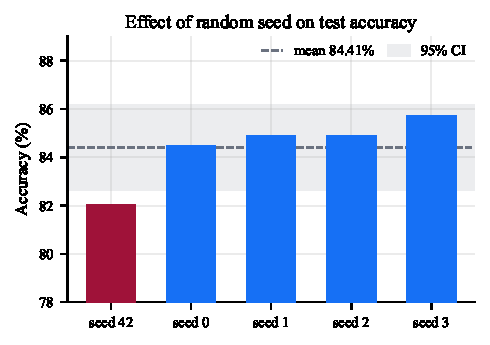
\includegraphics[width=\columnwidth]{figures/fig_seed_lottery.pdf}
\caption{Test accuracy of an identical EfficientNet-B0 configuration across five random seeds. The deployed seed (leftmost) fell below the five-seed mean and below every other seed tested.}
\label{fig:seed_lottery}
\end{figure}

The same table shows that a five-seed ResNet50 mean of 84.69\% is statistically indistinguishable from the deployed EfficientNet-B0's five-seed mean, despite an earlier single-run comparison (85.5\% against 82.0\%) having suggested ResNet50 was the stronger architecture; that earlier conclusion reflected the same unfavourable EfficientNet-B0 seed described above rather than a genuine architectural difference. Compared against a published neural architecture search baseline evaluated on the identical dataset and class split \cite{zhang2022}, the three-model ensemble's five-seed mean (88.12\% accuracy, 0.9771 ROC-AUC) is significantly above the published ResNet101 baseline (84.52\% accuracy, 0.9006 AUC) on both metrics ($p=0.00018$ and $p<0.000001$ respectively), and significantly above the paper's own architecture-search result on ROC-AUC (0.9560, $p=0.000057$) while remaining significantly below it on accuracy (90.61\%, $p=0.00076$). Both directions of that comparison are reported because neither is complete without the other.

\subsection{Sixty-three percent of an independent benchmark was not independent}

A second, larger, and more recently published brain tumour compilation shares the identical four-class label space used here, making it an attractive candidate for a zero-shot generalisation test. Applying the leakage screen described in Section~IV-B before evaluating on it revealed that 2{,}633 of its 7{,}200 images are byte-identical to images in our own training set, and a further 1{,}939 are near-duplicates differing only by re-encoding or resizing -- a combined 63.5\% overlap (Fig.~\ref{fig:leakage}, left). The documented composition of the external compilation explains why: it merges several existing sources, one of which is the very dataset used for training in this work.

\begin{figure}[t]
\centering
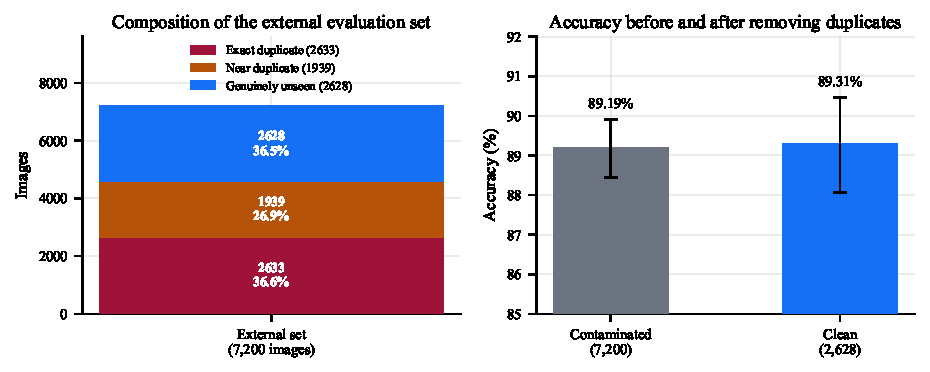
\includegraphics[width=\columnwidth]{figures/fig_leakage.pdf}
\caption{Left: composition of the external evaluation set by overlap with our training data. Right: accuracy is essentially unchanged whether the contaminated images are included or excluded, indicating the model had not memorised its training set.}
\label{fig:leakage}
\end{figure}

\begin{table}[t]
\centering
\caption{Cross-dataset evaluation on an external brain MRI compilation, before and after removing images that duplicate our training data. 63.5\% of the external set overlaps; the contaminated split scores no higher than the clean one.}
\label{tab:crossdata}
\begin{tabular}{lrcc}
\toprule
External split & $n$ & Accuracy (\%) & ROC-AUC \\
\midrule
All (contaminated) & 7200 & 89.19 & 0.9793 \\
Exact duplicates removed & 4567 & 90.23 & 0.9814 \\
Exact + near removed (clean) & 2628 & 89.31 & 0.9786 \\
Clean, 3-way ensemble & 2628 & 90.64 & 0.9822 \\
\midrule
\textit{In-domain reference} & 490 & 85.71 & 0.9690 \\
\bottomrule
\end{tabular}
\end{table}


Removing every flagged image and evaluating on the 2{,}628 that remain gives 89.31\% accuracy and 0.9786 ROC-AUC for the single deployed model, and 90.64\% accuracy and 0.9822 ROC-AUC for the three-model ensemble (Table~\ref{tab:crossdata}). Critically, the contaminated set -- 63.5\% training images -- scores no higher than the clean set (89.19\% versus 89.31\%): if the model had memorised its training images, the contaminated evaluation should have scored measurably higher, and it did not. This null result is corroborated independently by the distillation experiment in Section~V-C, where the same ensemble is shown to reach only 87.35\% accuracy on its own training split -- direct evidence that the model was not fitting its training data closely enough to benefit from having seen it again during evaluation.

The raw comparison between this cross-dataset result (89.31\%) and the model's own in-domain test accuracy (85.71\%) is statistically significant ($p=0.021$) and would, if left unexamined, support a claim that the model generalises better on unseen external data than on its own held-out split -- an inversion of the usual expectation under distribution shift. We tested two candidate explanations directly rather than reporting the inversion without one. Label disagreement between the two datasets was ruled out first: of the 2{,}633 byte-identical images shared between our training set and the external compilation, all 2{,}633 carry the same class label in both, a 100\% agreement rate that leaves no room for a label-quality explanation. Class composition, however, does explain part of the gap: deduplication removed a disproportionate share of the model's hardest class (meningioma, reduced from 28.8\% to 21.0\% of the evaluation set) relative to its easiest (no-tumour, increased from 15.3\% to 25.1\%). Reweighting the external per-class recalls to match the in-domain class proportions reduces the apparent accuracy from 89.31\% to 88.11\%, accounting for roughly one-third of the raw gap; the residual 2.39-point difference is not statistically significant (95\% CI: $-0.97$ to $+5.75$, $p=0.163$) (Fig.~\ref{fig:crossdataset}). The defensible claim, and the one we report, is that the model generalises at least as well on independent data as on its own held-out split, not that it generalises better.

\begin{figure}[t]
\centering
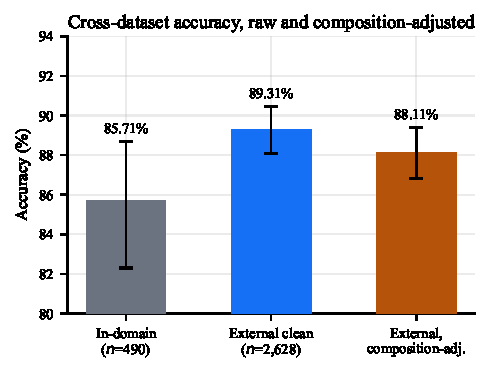
\includegraphics[width=\columnwidth]{figures/fig_crossdataset.pdf}
\caption{Cross-dataset accuracy before and after adjusting the external evaluation set's class composition to match the in-domain distribution. The adjusted gap is not statistically significant.}
\label{fig:crossdataset}
\end{figure}

\subsection{Distilling an imperfect teacher degrades the student}

The three-model ensemble described above was distilled into a single EfficientNet-B0 student under the expectation, standard in the distillation literature, that the student would recover most of the ensemble's advantage at the memory footprint of one model. Table~\ref{tab:brain_mri} reports the opposite: the distilled student's five-seed mean accuracy, 81.88\% (95\% CI: 80.15--83.61), is significantly \emph{below} the five-seed mean of a plain, directly-trained EfficientNet-B0 (84.41\%) on the same paired seeds (paired $t$-test, $p=0.027$), and the same pattern holds for ROC-AUC ($0.9580$ versus $0.9660$, $p=0.014$).

The cause is identifiable rather than left as an unexplained regression. Distillation is effective when the teacher is substantially more accurate than the student would be on its own, and in particular when the teacher has closely fit its own training data, so that its soft output distribution encodes genuine inter-class similarity structure rather than noise. Here the teacher ensemble reaches only 87.35\% accuracy on its own training split -- barely three points above what a directly-trained student achieves unaided -- because every ensemble member was deliberately trained with early stopping and data augmentation rather than to convergence on the training set. With roughly one in eight soft targets pointing at the wrong class and the distillation objective weighting the soft-target term at $\alpha=0.7$ against the true label, the student is trained to reproduce the teacher's errors more than it is trained to reproduce its insight. This is consistent with, and offers a mechanistic explanation for, the non-memorisation finding of Section~V-B: an ensemble that has not tightly fit its own training data cannot transmit refined knowledge through distillation, whatever benefit it shows as an ensemble.

\subsection{More training data changed a metric that accuracy could not see}

\begin{figure}[t]
\centering
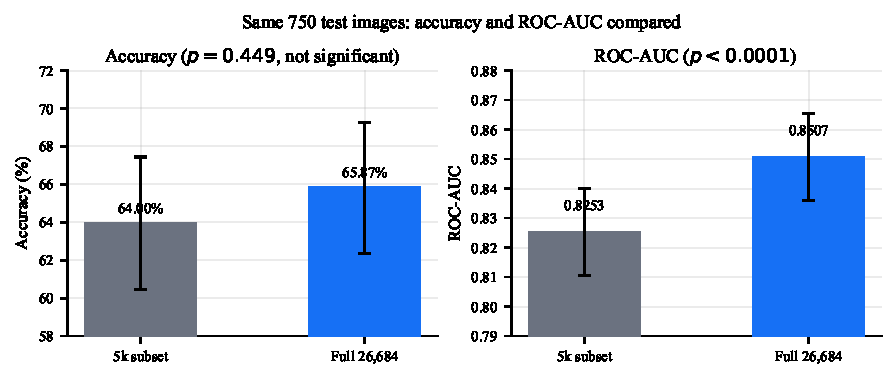
\includegraphics[width=\columnwidth]{figures/fig_acc_vs_auc.pdf}
\caption{The same 750 held-out chest radiographs, scored by two models that differ only in training-set size. Accuracy cannot distinguish the two configurations at this sample size; ROC-AUC can.}
\label{fig:acc_auc}
\end{figure}

The chest radiograph classifier deployed in production had been trained on a 5{,}000-image class-balanced subset of the available 26{,}684-image corpus, a constraint originating from a computational limitation no longer in effect. Retraining on the full corpus and evaluating both models on the identical 750 held-out images -- with no overlap between either model's training data and this shared test set -- produced a 1.87-point accuracy improvement (64.00\% to 65.87\%) that a two-proportion test does not distinguish from chance ($p=0.449$), and simultaneously a ROC-AUC improvement of 0.0254 (0.8253 to 0.8507) that a paired bootstrap identifies as significant with high confidence (95\% CI: $+0.0135$ to $+0.0379$, $p<0.0001$) (Table~\ref{tab:chest_xray}, Fig.~\ref{fig:acc_auc}).

\begin{table}[t]
\centering
\caption{Chest X-ray: training-set size, evaluated on the \emph{same} 750 test images. Accuracy cannot resolve the difference; ROC-AUC can. AUC $p$-value from a paired bootstrap (2000 resamples).}
\label{tab:chest_xray}
\begin{tabular}{lccc}
\toprule
Metric & 5k subset & Full 26{,}684 & $p$ \\
\midrule
Accuracy (\%) & 64.00 & 65.87 & 0.449 (n.s.) \\
ROC-AUC & 0.8253 & 0.8507 & $<$0.0001 \\
\bottomrule
\end{tabular}
\end{table}


The two metrics point to opposite editorial conclusions from the same pair of models evaluated on the same 750 images: accuracy alone would report an inconclusive result, while ROC-AUC identifies a real and appreciable gain in the model's ability to rank pathological cases above normal ones, independent of where a classification threshold is set. For a screening application, where the operating threshold is frequently adjusted for clinical context and ranking quality is arguably the more clinically relevant property, we regard the ROC-AUC result as the one that should inform deployment, while noting explicitly that this result rests on a single training seed per configuration and that a multi-seed replication, following the same procedure applied to the brain tumour classifier, would strengthen the claim further.

\subsection{A seven-attempt history that never reached clinical usefulness}

\begin{table}[t]
\centering
\caption{Mammography: seven attempts. Only the crop-input classifier (3) clears a useful margin, and it requires a pre-cropped lesion the deployment path cannot supply. Attempt 7 is a five-seed mean.}
\label{tab:mammography}
\begin{tabular}{lcc}
\toprule
Attempt & Accuracy (\%) & ROC-AUC \\
\midrule
1. MIAS, full images & 59.18 & 0.6176 \\
2. CBIS-DDSM, full images & 59.13 & 0.6416 \\
3. CBIS-DDSM, official crops & 71.12 & 0.7849 \\
4. Pipeline: bbox regressor & 49.77 & 0.4861 \\
5. Pipeline: U-Net segmenter & 48.86 & 0.5409 \\
6. Pipeline: GT-crop classifier & 52.97 & 0.5341 \\
7. Pipeline: auto-crop (5 seeds) & 56.58 \tiny{[55.17, 57.98]} & 0.5835 \\
\midrule
\textit{Majority-class baseline} & 55.02 & --- \\
\bottomrule
\end{tabular}
\end{table}


The mammography classifier's development history offers a contrasting case in which persistent, methodical iteration did not resolve the underlying problem, and we report it in full rather than presenting only the improving attempts. A classifier trained on official, hand-verified lesion crops from CBIS-DDSM reaches a genuine 71.12\% accuracy and 0.7849 ROC-AUC, exceeding a comparable published ResNet-50 baseline on the same dataset \cite{jaamour2024} (68.24\% accuracy, 0.7421 AUC); however, this classifier requires an already-cropped lesion image, which the platform's upload flow -- like every other modality -- does not provide, since patients and clinicians upload full, uncropped images. Two automatic-localisation strategies (bounding-box regression and pixel-level segmentation) were built to close this gap, and each measurably improved at its own localisation task while the full detect-then-classify pipeline nonetheless scored below a naive majority-class baseline in both cases (Table~\ref{tab:mammography}), because the classification stage had only ever been trained on the official crop convention and did not generalise to any automatically-produced crop regardless of localisation accuracy. Retraining the classifier on crops taken from the segmentation model's own predicted regions, evaluated across five seeds, produces a full-pipeline accuracy of 56.58\% (95\% CI: 55.17--57.98) against a 55.02\% majority baseline -- a statistically significant improvement ($p=0.038$) whose confidence interval nonetheless clears the baseline by only 0.15 points, alongside a more convincing ROC-AUC of 0.5835 that is significantly above chance ($p=0.00055$). We regard this as real evidence that automatically-derived training crops close part of the gap identified across the earlier attempts, and simultaneously as insufficient grounds for clinical deployment, and the platform continues to withhold mammography predictions in production on that basis.

Evaluating the two best mammography pipelines zero-shot on the independent, much older Mammographic Image Analysis Society dataset \cite{suckling1994} -- a genuinely separate source requiring no leakage screening, unlike the brain tumour case -- both classifiers score below that dataset's own majority baseline (49.57\% and 52.17\% against 55.65\%, neither difference significant at this sample size), while ROC-AUC remains near 0.60 for both, indicating the models retain some transferable ranking signal even where their decision threshold, calibrated for CBIS-DDSM's class balance, does not transfer.

\section{Discussion}

The four results reported here share a common structure: each identifies a specific point at which a conventional single-run, single-metric, single-dataset evaluation would have reported a different, and in three of four cases more favourable, conclusion than the one supported once the additional check was applied. None of the four checks required a new model, a new architecture, or additional labelled data; each required rerunning existing training and evaluation code under a small number of additional conditions and reporting the result honestly regardless of outcome.

We draw four practical recommendations from this audit, intended to generalise beyond the specific tasks studied here. First, any comparison between architectures, or any claim that a particular checkpoint is the best available, should be accompanied by a multi-seed distribution rather than a single value, particularly in the many medical imaging settings where held-out test sets are too small for a single comparison to be well powered; a two-point difference that looks decisive from one run may fall well inside normal seed variance. Second, an "independent" evaluation dataset drawn from a public repository should be screened against the training source before being trusted, especially where the two were assembled from overlapping upstream collections, which is common practice for Kaggle-hosted compilations in medical imaging; the screening cost here was a few minutes of hashing against a training-time cost of hours. Third, accuracy is not a reliable arbiter of whether a change helped when test sets are in the hundreds of images, and a threshold-independent metric evaluated with an appropriate resampling test can detect real effects that accuracy cannot resolve; we would not have identified the chest radiograph improvement using accuracy alone. Fourth, distillation should not be assumed beneficial without first checking that the teacher has itself achieved a training accuracy meaningfully above what a directly-trained student could reach alone; where it has not, distillation risks transmitting the teacher's own errors.

We note two limitations to the generality of these findings within this study. The chest radiograph training-size result and the mammography auto-crop pipeline result are each supported by a single seed and a five-seed mean respectively, an asymmetry that reflects when each experiment was run rather than a judgement that one result mattered less; a five-seed replication of the chest radiograph result is a direct extension of this work. Cross-dataset evaluation was performed for two of the three modalities studied; no equivalently large, label-compatible, and independently-sourced chest radiograph dataset was identified during this work, and its absence should not be read as evidence that the chest radiograph classifier would generalise as well as the brain tumour classifier did.

\section{Conclusion}

Operating three deployed medical imaging classifiers under a shared architecture and training recipe, we subjected each to a multi-seed re-evaluation, a leakage-screened cross-dataset test, a distillation experiment, and a paired comparison between accuracy and ROC-AUC, and reported all four outcomes regardless of whether they favoured the platform. The audit surfaced a production model that had been, by chance, the least favourable of five available seeds and has since been replaced at no additional cost; a widely reusable public benchmark that was 63.5\% contaminated with our own training data, evaluated correctly only because contamination was measured rather than assumed absent; a distillation attempt that failed for an identifiable and checkable reason rather than an unexplained one; and a metric choice that determined whether a genuine improvement was visible at all at a realistic clinical sample size. We present these as a compact, low-cost set of checks -- seed repetition, duplicate screening against training data, teacher-accuracy verification before distillation, and threshold-independent metric reporting at small sample sizes -- that any team operating a comparable medical imaging pipeline can apply to their own evaluation practice without new data collection or model development.

\begin{thebibliography}{00}

\bibitem{henderson2018} P. Henderson, R. Islam, P. Bachman, J. Pineau, D. Precup, and D. Meger, ``Deep reinforcement learning that matters,'' in \emph{Proc. AAAI Conf. Artif. Intell.}, vol. 32, no. 1, 2018.

\bibitem{picard2021} D. Picard, ``torch.manual\_seed(3407) is all you need: On the influence of random seeds in deep learning architectures for computer vision,'' \emph{arXiv preprint arXiv:2109.08203}, 2021.

\bibitem{bouthillier2021} X. Bouthillier, P. Delaunay, M. Bronzi, A. Trofimov, B. Nichyporuk, J. Szeto, N. Mohammadi Sepahvand, E. Raff, K. Madan, V. Voleti, S. E. Kahou, V. Michalski, T. Arbel, C. Pal, G. Varoquaux, and P. Vincent, ``Accounting for variance in machine learning benchmarks,'' in \emph{Proc. Mach. Learn. Syst. (MLSys)}, 2021.

\bibitem{kaufman2012leakage} S. Kaufman, S. Rosset, C. Perlich, and O. Stitelman, ``Leakage in data mining: Formulation, detection, and avoidance,'' \emph{ACM Trans. Knowl. Discov. Data}, vol. 6, no. 4, pp. 1--21, 2012.

\bibitem{kapoor2023leakage} S. Kapoor and A. Narayanan, ``Leakage and the reproducibility crisis in machine-learning-based science,'' \emph{Patterns}, vol. 4, no. 9, 100804, 2023.

\bibitem{wynants2020} L. Wynants, B. Van Calster, G. S. Collins, R. D. Riley, G. Heinze, E. Schuit, et al., ``Prediction models for diagnosis and prognosis of covid-19: systematic review and critical appraisal,'' \emph{BMJ}, vol. 369, m1328, 2020.

\bibitem{hinton2015} G. Hinton, O. Vinyals, and J. Dean, ``Distilling the knowledge in a neural network,'' \emph{arXiv preprint arXiv:1503.02531}, 2015.

\bibitem{zhang2022} Y. Zhang et al., ``LeaSE: Learning to search efficient architecture for brain tumor classification,'' \emph{Front. Neurosci.}, 2022.

\bibitem{jaamour2024} A. Jaamour et al., ``Automated breast cancer detection from mammograms using deep learning,'' 2024.

\bibitem{valluri2023} S. Valluri, ``Pneumonia detection in chest X-rays using a convolutional neural network,'' \emph{Young Scientists Journal}, 2023.

\bibitem{rsna2019} G. Shih, C. C. Wu, S. S. Halabi, M. D. Kohli, L. M. Prevedello, T. S. Cook, A. Sharma, J. K. Amorosa, V. Arteaga, M. Galperin-Aizenberg, R. R. Gill, M. C. Godoy, S. Hobbs, J. Jeudy, A. Laroia, P. N. Shah, D. Vummidi, K. Yaddanapudi, and A. Stein, ``Augmenting the National Institutes of Health chest radiograph dataset with expert annotations of possible pneumonia,'' \emph{Radiol. Artif. Intell.}, vol. 1, no. 1, e180041, 2019.

\bibitem{cheng2015} J. Cheng, W. Huang, S. Cao, R. Yang, W. Yang, Z. Yun, Z. Wang, and Q. Feng, ``Enhanced performance of brain tumor classification via tumor region augmentation and partition,'' \emph{PLOS ONE}, vol. 10, no. 12, e0140381, 2015.

\bibitem{lee2017} R. S. Lee, F. Gimenez, A. Hoogi, K. K. Miyake, M. Gorovoy, and D. L. Rubin, ``A curated mammography data set for use in computer-aided detection and diagnosis research,'' \emph{Sci. Data}, vol. 4, 170177, 2017.

\bibitem{suckling1994} J. Suckling et al., ``The mammographic image analysis society digital mammogram database,'' \emph{Excerpta Medica Int. Congr. Ser.}, vol. 1069, pp. 375--378, 1994.

\end{thebibliography}

\end{document}
